%
% $File: report.tex
% $Date: Thu Jun 13 01:47:12 2013 +0800
% $Author: Xinyu Zhou <zxytim@gmail.com>
%

\documentclass{article}
\usepackage{fontspec}
\usepackage{url,amsmath,amssymb,verbatim}
\let\mathdollar\relax
\usepackage{MnSymbol}
\let\mathdollar\relax
\usepackage{pdfpages}
\usepackage{zhspacing}
\zhspacing
\usepackage{listings}
\usepackage[hyperfootnotes=false,colorlinks,linkcolor=blue,anchorcolor=blue,citecolor=blue]{hyperref}
\usepackage[sorting=none]{biblatex}
%\usepackage[dvips]{graphicx}
%\usepackage{graphicx}
%\usepackage{minted}
\usepackage{indentfirst}
\usepackage{cases}
\usepackage{environ}
\usepackage{array}
\usepackage[top=1in, bottom=1in, left=1.25in, right=1.25in]{geometry}
%\usepackage{tikz}
%\usepackage{dot2texi}

\usepackage{dirtree}
%% $File: mint-defs.tex
% $Date: Tue Apr 03 00:49:58 2012 +0800
% $Author: Xinyu Zhou <zxytim@gmail.com>

\newcommand{\inputmintedConfigured}[3][]{\inputminted[fontsize=\footnotesize,
	label=#3,linenos,frame=lines,framesep=0.8em,tabsize=4,#1]{#2}{#3}}

\newcommand{\txtsrc}[2][]{\inputmintedConfigured[#1]{text}{#2}}
\newcommand{\txtsrcpart}[4][]{\txtsrc[firstline=#3,firstnumber=#3,lastline=#4,#1]{#2}}

\newcommand{\cppsrc}[2][]{\inputmintedConfigured[#1]{cpp}{#2}}
\newcommand{\cppsrcpart}[4][]{\cppsrc[firstline=#3,firstnumber=#3,lastline=#4,#1]{#2}}



%\renewcommand{\baselinestretch}{1.62} 
\usepackage{setspace}

\newcommand{\figref}[1]{\hyperref[fig:#1]{Figure\ref*{fig:#1}}}
\newcommand{\tableref}[1]{\hyperref[table:#1]{Table\ref*{table:#1}}}
\newcommand{\centerize}[1]{\begin{center} #1 \end{center}}

\newcommand{\cmd}[1]{{\it #1}}
\newcommand{\ccmd}[1]{\centerize{\cmd{#1}}}


\title{数字逻辑实验彩灯实验报告}
\author{周昕宇 ID: 2011011252\\李其乐 ID: 2011011247\\ Dept. CST, THU}
\date{\today}

\addbibresource{refs.bib}
\begin{document}
\maketitle
\tableofcontents
\clearpage

\section{游戏简介}
\begin{spacing}{1.62}
	我们一共制作了两个游戏:
	\begin{itemize}
		\item {\bf 是男人就下一百层 }

			游戏场景由屏幕上的一些平台和一个游戏组成,平台垂直于水平线,
			游戏角色是垂直平台的1*2的矩形。平台定时缓慢右移;
			当游戏角色不在平台上时则以较快的速度定时左移,
			而游戏角色在平台上时则与平台同步右移。
			当游戏角色达到屏幕左端游戏结束;
			如果游戏角色随着平台下落达到屏幕右端,则游戏亦结束。
			游戏结束后屏幕将全亮。

			玩家可以通过挥动手来控制游戏角色的上下移动,
			也可以通过点击rst键来重启游戏,游戏重启后屏幕会暂时全暗,
			之后会重新显示游戏的开始画面。

		\item {\bf 乒乓球}

			游戏场景由两个球拍和一个球组成,球拍都平行于水平线,是1*3的矩形;球由一个点构成。两个玩家可以操控各自球拍在屏幕的上或下端左右移动。开始游戏时,发球权属于处在屏幕上端的球拍。球碰到屏幕的左右端点或碰到球拍会反弹。如果球达到屏幕下端,操控上端的玩家获胜,此时屏幕全亮;如果球达到屏幕上端,操控下端球拍的玩家获胜,此时屏幕全暗。
			玩家可以通过k4 k5键操控上端的球拍,通过k0
			k1键操控下端的球拍。Rst键是重新开始,clk键是发球
	\end{itemize}


	由于逻辑单元的限制,以及乒乓球游戏的优化不足导致其无法使用超声波距离传感器进行用户交互。
\end{spacing}

\section{设计}

\begin{spacing}{1.62}
整个项目由三个模块构成:显示屏幕,超声波距离传感器,及游戏逻辑。
顶层entity为wave\_your\_hand。entity结构如下
\dirtree{%
.1 wave\_your\_hand.
.2 man(游戏逻辑).
.3 man\_on\_a\_plat(游戏角色是否在某一个平台上).
.3 pos\_has\_a\_plat(屏幕某位置是否某平台覆盖).
.2 screen(显示屏幕).
.3 LED(LED模块).
.2 uss(超声波距离传感器,Ultra Sonic Sensor).
}

设计中最大的挑战为MAX II EPM240芯片所提供逻辑单元过少,需要优化设计,使之
消耗更少的逻辑单元。

\end{spacing}
\subsection{显示屏幕}
\begin{spacing}{1.62}
显示屏幕由两个LED实体构成。

	LED实体的接口为:
	\begin{itemize}
		\item clk: in std\_logic
			
			LED控制时钟

		\item enable: in std\_logic

			使能端,为更高层screen实体使用

		\item row, col: in integer range 0 to 7

			需要显示的行与列

		\item led\_data: in std\_logic

			显示的数据

		\item output: out std\_logic\_vector(0 to 23)

			输出控制led的信号

	\end{itemize}

	其工作方式为:当使能端为'1'且clk负边沿触发时,根据row, col, led\_data计算出
	相应的output信号,从而控制一个二极管的暗灭。



屏幕接口为: 
\begin{itemize}
	\item clk, led\_data: in std\_logic
		时钟与数据输入
	\item trig: out std\_logic
	\item row\_out: out integer range 0 to 7
	\item col\_out: out integer range 0 to 15
	\item output: out std\_logic\_vector 0 to 47
\end{itemize}

屏幕控制两个LED灯,output的下标0至23部分接入第一个LED,
24至47部分接入第二个LED。4个时钟脉冲为一个工作周期。该实体在相应的时钟脉冲序号下的工作如下:
\begin{enumerate}
	\item trig设为'1',给外部逻辑的正边沿触发信号。外部逻辑检测到该信号后根据row\_out与col\_out(行与列)计算出需要显示信号。
	\item 内部LED时钟信号led\_clk设为'1',触发LED灯进行显示。 
	\item row 与 col响应增加到下一个像素点,且trig设为'0',结束触发信号。 
	\item led\_clk设为'0'
\end{enumerate}

\end{spacing}
\subsection{超声波距离传感器}

\begin{spacing}{1.62}
所使用的超声波距离传感器为HC-SR04,其时序工作图如下:

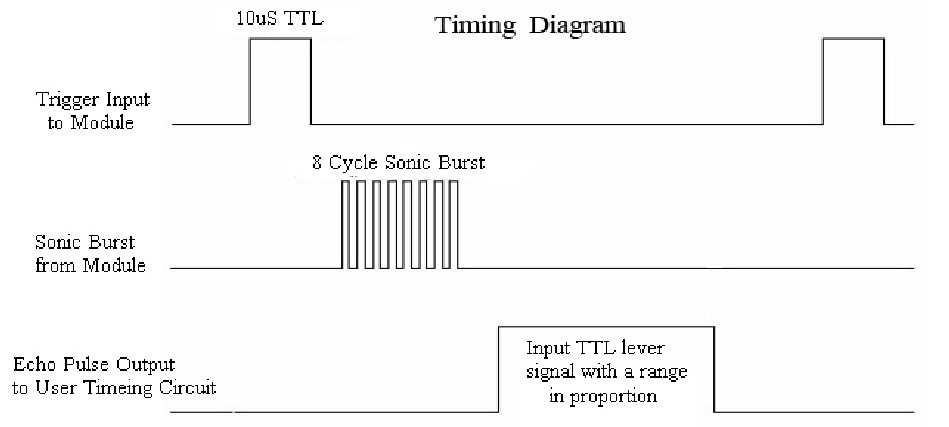
\includegraphics[width=\textwidth]{res/uss-timing.png}

该实体接收2MHz的时钟信号,每25ms为一个工作周期。
每个工作周期内给传感器10us的触发信号,然后等待其返回信号,根据2MHz的时钟频率及
传感器返回高电平信号的时间及声速计算距离。
\end{spacing}

\subsection{游戏逻辑}

\begin{spacing}{1.62}
\begin{itemize}
	\item {\bf 是男人就下一百层}

		游戏处于四个状态中的其中一个:RESET, INIT, GAMING, GAME\_OVER。

		游戏中有三个平台,分别用2个整数表示其中心坐标。平台上升及角色下落分别用不同的时钟频率,并且
		保证其不会同时触发。

		平台上升条件或角色下落条件触发后,进行相应的逻辑处理。

	\item {\bf 乒乓球}

		玩家的指令输入和游戏逻辑控制在同一个entity(blocks)中,因此游戏只需要结合逻辑控制和屏幕显示的模块,具体方法大同小异。
		正是由于游戏设计采用逻辑控制和屏幕显示相分离的设计方法,而且统一了各个模块的接口。所以两游戏的screen模块可以复用,
		进而减少了工作量。

\end{itemize}
\end{spacing}

\section{项目分工}
\begin{itemize}
	\item {\bf 周昕宇}:
		
		器件选择,基础架构设计及实现,是男人就下一百层游戏逻辑实现及优化。

	\item {\bf 李其乐}:

		乒乓球游戏实现,是男人就下一百层功能完善。
\end{itemize}


\section{实验用器件}
\begin{itemize}
	\item 超声波距离传感器HC-SR04 一个
	\item 8x8灯阵1588ABEG 两个
	\item CPLD芯片 MAXII EMP240T 一个
\end{itemize}
\section{关键技术分析}
\begin{spacing}{1.62}

项目的核心问题为芯片逻辑单元数量过少,逻辑实现比较困难。由于有灯阵,有传感器,
并且还有相对复杂的游戏逻辑,在一块240逻辑单元上实现遇到极大的挑战。为此,我们
对于代码的每一部分都进行了大量测试,使用不同的设计方法进行实现并且验证,而后进行
逻辑单元使用数量的优化。

\begin{itemize}
	\item 整体的优化
			对于所有整数类型都指定范围,且在时钟脉冲计数加法中让其自然溢出。
	\item 屏幕显示
		显示屏幕的设计理念为:无状态。即在任意时刻无法得知人因为视觉暂留所看到的屏幕的样子。
		这是因为若要存储整个屏幕,逻辑单元消耗的数量将会大大增加。

		由于为了节省逻辑单元,采取了一个时钟内只亮一个灯的设计,从而导致每个二极管
		通电时间过短,LED灯较暗的问题。而由于row, col信号为screen实体控制
		发出,保证了按照一定的行列顺序,为了使得LED灯更亮,在LED实体内对一行的数据做了缓存:
		如果当前行未改变,则增加增加修改量。实验表明LED的亮度有大幅提升。

	\item 超声波距离传感器
		由于游戏中该器件用于控制角色左右移动,故输出只需-1、0、+1,分别表示左移、停止、右移。
		测试表明,HC-SR04对3至12厘米区间内敏感度较高,故将此区间作为有效区间,均分为左、中、右
		三部分。

		并且为了避免取模运算,采取了计数的方式累加输出。

	\item 游戏逻辑
		由于屏幕显示及超声波距离传感器都已经经过充分优化,两部分单独加在一起一共只占用65个逻辑单元,
		但不排除由于部分信号未使用而导致编译时优化中将其优化省去,但也从一个侧边表明
		逻辑单元的主要消耗在于游戏逻辑。为了能在240个逻辑单元内实现游戏逻辑,以{\bf 是男人就下一百层}为例,
		我们尝试了如下方法:

		\begin{itemize}
			\item {\bf 去掉屏幕实体,直接操作屏幕输出}。
				
				我们期望由于逻辑中间层的减少,从而让逻辑单元消耗更少,
				但实验表明,此方法会将大量逻辑单元消耗在对于std\_logic\_vector的整体赋值上,没有有效
				地减少逻辑单元使用数量。

			\item {\bf 更改游戏数据表示方法,用一个大小为128的数组作为平台表示}。

				这样做的好处有
				\begin{enumerate}
					\item 角色是否在平台上的逻辑判断变得简洁
					\item 平台数量和逻辑单元消耗几乎无关(初始化时可能相关)
					\item 平台上升只需要位移操作即可
					\item 屏幕显示逻辑也变得简洁
				\end{enumerate}
				但同时也带来了劣势: 由于数组过大,初始化占用逻辑单元太多。

				首先,我们尝试先将数组全部赋值为'0',再把少数为'1'的部分单独赋值,
				但这样逻辑单元消耗依然很大。

				经过查找资料,我们尝试使用MAX II芯片自带的{\bf User Flash Memory(UFM)}进行数据存储,并且
				在游戏初始化时读入数据。我们尝试了不同的UFM Megafunction: {\bf ALTUFM\_PARALLEL}
				及 {\bf ALTUFM\_SPI},其中{\bf ALTUFM\_SPI}尝试了其{\bf Base mode}和{\bf Extended mode},
				且都为Read only的访问模式,以期
				Megafunction所使用的逻辑单元加上使用UFM所耗逻辑单元的数量小于直接初始化数组
				消耗的数量。

				但实验结果表明,{\bf ALTUFM\_PARALLEL}由于需要对数组进行批量赋值而
				消耗逻辑单元较多;{\bf ALTUFM\_SPI}的{\bf Base mode}虽然本身使用逻辑单元较多,但一次处理数据
				量较少,{\bf Extended mode}虽然本身逻辑单元较少,但其一次处理数据量较大。
				最终没有一个组合能达到我们期望的效果。

				而反观需求,我们只初始化最开始的平台布局而不是需要大量的数据,比如
				播放动画或者音乐,故在几天的尝试后,
				最后遗憾地得出结论,此方法不适合使用。

			\item {\bf 优化游戏逻辑,组合逻辑单独计算}。

				在各种尝试后,最后的数据表示方式为存储平台本身坐标及角色坐标,
				但这样带来的问题为,游戏本身的逻辑变得更加复杂
				\begin{enumerate}
					\item 需要判断角色是否位于某个平台上,需要枚举平台,且枚举平台所站的3个格子。
					\item 显示时需要判断该像素是否有平台,也需要枚举平台及其所站的格子
				\end{enumerate}
				经测试,其逻辑单元消耗数量和用大小为128的额数组表示平台背景相差无几。
				
				在焦头烂额之际,我们推测,逻辑单元的消耗主要在于复杂的时序逻辑在电路
				实现时会变得比较复杂,而组合逻辑则非常简单。
				而我们欣喜地发现,这两个问题由于都只涉及组合逻辑判断,和时序逻辑无关,
				故对于这两个需要计算的数据,形式化其逻辑后用单独的entity进行组合逻辑计算,
				从而使逻辑单元使用数量大幅减少,一举跃进240个逻辑单元的边缘,一共使用了228个
				逻辑单元。最后加上一些过场效果,240个逻辑单元刚好用完。

		\end{itemize}

\end{itemize}

\section{总结}
\begin{spacing}{1.62}
	在购买的传感器到货后,我们只耗费一天便做出了整个游戏的原型,但由于逻辑单元的限制,
	我们进行了连续长达6天的优化过程,所用尝试过的优化方法并未列尽(如屏幕及传感器的逻辑单元优化)。
	期间我们查阅大量资料,做了大量实验,大量的调研和学习同时也增长了我们VHDL的知识,大大加深了我们对
	硬件的理解。
	
	最后功夫不负有心人,我们成功完成了项目。但由于芯片能力的限制,计划中的功能并
	未能完全实现。

	通过这次实验,我们感受到了数字逻辑电路的强大以及其不足,对数字逻辑电路的理解也大大增加。

\end{spacing}

\end{spacing}
%\clearpage

%\printbibliography

\end{document}

